% !TeX spellcheck = en_US

\documentclass[a4paper,oneside,11pt]{memoir}

\usepackage[utf8]{inputenc} % Input encoding - Depending on the editor
\usepackage{lmodern} % Modern LaTeX font
\usepackage[english]{babel} % Language package <- CHANGE LANGUAGE HERE
\usepackage[T1]{fontenc} % Hyphenation
\usepackage{fix-cm} % Fix for cm

\usepackage{xcolor} % To define colors
% Used to generate links, can be removed for final version
\usepackage[hidelinks]{hyperref}
%used for \cref
\usepackage{cleveref}
\usepackage{lipsum} % Debugging text

\usepackage{sansmath} % Font for floats
%\usepackage{listings}

\newcommand{\shellcmd}[1]{\\\texttt{\footnotesize\# #1}}

% *** CITATION PACKAGE ***
\usepackage{cite}

% *** GRAPHICS RELATED PACKAGES ***
%
\usepackage[pdftex]{graphicx}
%   declare the path(s) where your graphic files are
\graphicspath{{../pdf/}{../jpeg/}}
%   and their extensions so you won't have to specify these with
%   every instance of \includegraphics
\DeclareGraphicsExtensions{.pdf,.jpeg,.png}

\usepackage{pgfplots}
\pgfplotsset{compat=1.8}
\usepgfplotslibrary{statistics}

\usepackage{filecontents}

\usepackage[caption=false,font=normalsize,labelfont=sf,textfont=sf]{subfig}



% *** PDF, URL AND HYPERLINK PACKAGES ***

\usepackage{url}


\newsubfloat{figure} % Declaring subfloats of figures
\newsubfloat{table} % Declaring subfloats of tables
\captionnamefont{\sffamily\sansmath\small} % Fontstyle of caption
\captiontitlefont{\sffamily\sansmath\small} % Fontsyle of caption

\definecolor{ase_blue}{RGB}{10,55,136} % The ASE blue color

%---------------------------------------------------------------------------%
%---------------------------- MARGIN CONTROL -------------------------------%
%---------------------------------------------------------------------------%
\setlrmarginsandblock{3.5cm}{2.5cm}{*}
\setulmarginsandblock{3cm}{*}{1.2}
\checkandfixthelayout[nearest]
\setlength{\evensidemargin}{\oddsidemargin}

%--------------------------------------------------------------------------%
%------------------------- FRONTPAGE - PROPERTIES -------------------------%
%--------------------------------------------------------------------------%
\usepackage{soul} % Letterspace package
\sodef\an{}{0.05em}{.5em plus.6em}{1em plus.1em minus.1em}
\newcommand\stext[1]{\an{\scshape#1}}
\newcommand{\logoHuge}{\fontsize{0.55cm}{0.8cm}\selectfont}
\newcommand{\SuperHuge}{\fontsize{1.2cm}{1.8cm}\selectfont}


%--------------------------------------------------------------------------%
%------------------------- PAGESTYLE - PROPERTIES -------------------------%
%--------------------------------------------------------------------------%
%\renewcommand{\chaptermark}[1]{\markboth{\MakeUppercase{#1}}{}}

\makepagestyle{ase_report}
\makeoddhead{ase_report}{}{\small\sffamily\leftmark}{}
\makeoddfoot{ase_report}{}{}{\small\sffamily\thepage}

\makeatletter
\makepsmarks{ase_report}{%
	\renewcommand\chaptermark[1]{%
		\markboth{%
			\ifnum \value{secnumdepth} > 1
			\if@mainmatter % 
			\@chapapp\ \thechapter. \ %
			\fi
			\fi
			##1}{}}
	\renewcommand\lofmark{\markboth{\listfigurename}{\listfigurename}}%
	\renewcommand\lotmark{\markboth{\listtablename}{\listtablename}}%
	\renewcommand\bibmark{\markboth{\bibname}{\bibname}}%
	\renewcommand\indexmark{\markboth{\indexname}{\indexname}}%
	\renewcommand\sectionmark[1]{\markright{##1}}%
	\renewcommand\subsectionmark[1]{\markright{##1}}%
	\renewcommand\subsubsectionmark[1]{\markright{##1}}%
}

\copypagestyle{plain}{ase_report}
\makeoddhead{plain}{}{}{}
\makeoddfoot{plain}{}{}{\small\sffamily\thepage}

\pagestyle{ase_report}
\aliaspagestyle{chapter}{plain}



%--------------------------------------------------------------------------%
%--------------------- HEADING - SECTION ----------------------------------%
%--------------------------------------------------------------------------%
\newcommand{\ruledsec}[1]{%
	\Large\bfseries\sffamily\raggedright #1
	\color{ase_blue}\nopagebreak\rule[15pt]{\textwidth}{1.0pt}} % Section with ruler
\setsecheadstyle{\ruledsec} % Define section head style

\setfloatlocations{figure}{htp}
\setfloatlocations{table}{htp}



%--------------------------------------------------------------------------%
%--------------------- HEADING - SUBs-SECTION -----------------------------%
%--------------------------------------------------------------------------%
\addtocounter{secnumdepth}{2} % Depth numbering

\setsubsecheadstyle{\large\bfseries\sffamily\raggedright}
\setsubsubsecheadstyle{\bfseries\sffamily\raggedright}

\setsechook{\hangsecnum} % Hang the section number in margin
\setsubsechook{\defaultsecnum} % Don't do this on the subsections
\setsubsubsechook{\defaultsecnum}
\setaftersecskip{5pt} % Default skip between the section and text

%--------------------------------------------------------------------------%
%------------------------- TOC - PROPERTIES -------------------------------%
%--------------------------------------------------------------------------%
\raggedbottomsectiontrue % The page may not be strected on page breaks
\setsecnumdepth{subsection} % Set section depth in the TOC
\maxsecnumdepth{subsection} % Max of section depth in the TOC
\settocdepth{subsection} % Up to and including subsection

\setlength{\cftbeforechapterskip}{1.0em plus 0.1em minus 0.1em} % Space from chapters
%\chapterprecistoc{Text in TOC}

\addto\captionsenglish{
	\renewcommand*{\cftchaptername}{Chapter{\space}}
	\renewcommand*{\cftfigurename}{Fig.{\space}}
	\renewcommand*{\contentsname}{Table of Contents}
	\renewcommand*{\abstractname}{Abstract}
	\renewcommand*{\listfigurename}{List{\space}of{\space}Figures}
	\renewcommand*{\listtablename}{List{\space}of{\space}Tables}
	\renewcommand*{\appendixtocname}{Appendices}
	\renewcommand*{\appendixpagename}{Appendices}
}

\addto\captionsdanish{
	\renewcommand*{\cftchaptername}{Kapitel\space}
	\renewcommand*{\cftfigurename}{Fig.\space}
	\renewcommand*{\abstractname}{Resumé}
	\renewcommand*{\contentsname}{Indholdsfortegnelse}
	\renewcommand*{\listfigurename}{Liste{\space}af{\space}Figurer}
	\renewcommand*{\listtablename}{Liste{\space}af{\space}Tabeller}
	\renewcommand*{\appendixtocname}{Appendikser}
	\renewcommand*{\appendixpagename}{Appendikser}
}


%--------------------------------------------------------------------------%
%------------------------- CHAPTER STYLE ----------------------------------%
%--------------------------------------------------------------------------%
\makechapterstyle{ase_chapterstyle}{
	\setlength{\beforechapskip}{30pt}
	\setlength{\afterchapskip}{1.5cm}
	\renewcommand*{\printchaptername}{}
	\renewcommand*{\chapnumfont}{\normalfont\sffamily\bfseries\fontsize{60}{0}\selectfont}
	\renewcommand*{\printchapternum}{
		\flushright
		\begin{tikzpicture}
		\draw[fill,color=ase_blue] (0,0) rectangle (2cm,2cm);
		\draw[color=white] (1cm,1cm) node { \chapnumfont\thechapter };
		\end{tikzpicture}
	}
	\renewcommand*{\chaptitlefont}{\normalfont\sffamily\Huge\bfseries\color{black}}
	\renewcommand*{\printchaptertitle}[1]{%
		\raggedright\chaptitlefont\parbox[t]{\textwidth}{\raggedright##1}}
}

\chapterstyle{ase_chapterstyle}


\hyphenation{op-tical net-works semi-conduc-tor}

\hypersetup{pdfauthor={Stefan~Krause-Kj\ae r, Thomas Thisgaard Steffensen,Theis Nickelsen}, pdftitle={Context-Aware Authentication},
	pdfsubject={Using Bluetooth Low Energy}}


\begin{document}

\title{Context-Aware Authentication \\ Using Bluetooth Low Energy}

\author{Stefan~Krause-Kj\ae r\\
        Thomas Thisgaard Steffensen\\
        and \\
        Theis Nickelsen% <-this % stops a space
}

\newcommand{\buildBoxPlot}[5]{
	\addplot+[
	blue,
    solid,
	boxplot prepared={
		median= #1,
		upper quartile=#2,
		lower quartile=#3,
		upper whisker=#4,
		lower whisker=#5
	},
	] coordinates {};
	
}

\frontmatter
% Frontpage - Titlingpage from Memoir class 
\begin{titlingpage}
  
  \thispagestyle{empty}
  
  % Define the colourbar on the frontpage
  \begin{tikzpicture}[remember picture,overlay]
    \coordinate [below=2.5cm] (midpoint) at (current page.north);

    \node [name=colourbar,
    anchor=base,
    fill=ase_blue,
    text = white,
    minimum width=\paperwidth,
    minimum height=1cm] at (midpoint) {\logoHuge{\textsc{{Aarhus School Of
            Engineering}}}};

    % Define the point where the logo will go
    \coordinate [right=4cm] (ase_logo) at (colourbar.west);

    % Set coordinate system origin
    \begin{scope}[shift=(ase_logo)]
      % Draw the outline
      \filldraw [white] (1.2,0.85) -- (-1.6,0.85) -- (-2.3,-0.85) -- (1.2,-0.85) --cycle;
      % Include the logo
      \node [xshift=-0.5cm]{
\includegraphics[width=3cm]{img/ase_logo.png}};
    \end{scope}
  \end{tikzpicture}

  % Temporary center margins
  \begin{adjustwidth}{-0.5cm}{0cm}
    \vspace*{\stretch{0.5}}
    \centering
    { \setlength{\baselineskip}{32pt}
      {\SuperHuge \stext{Context-Aware Authentication} 
      }\par
      \stext{Using Bluetooth Low Energy}
      \par\vspace*{4\onelineskip}
      \par
%      
\includegraphics[width=10cm]{img/ase_logo}
      \par\vspace*{4\onelineskip}
      \textbf{\stext{Engineering Research and Development Project}}\par
      \par\vspace*{2\onelineskip}
      % Make a table to make the --- align
      \begin{center}
        \begin{tabular}{lcl}
          \large\stext{Stefan~Krause-Kj\ae r, } & \large\stext{---} &
          \large\stext{201300256} \\ [1ex]
          % To use danish letters with the UTF8 and soul package
          % we type \o = ø , \ae = æ, \aa = å, \AA = Å, etc.
          \large\stext{Thomas Thisgaard Steffensen} & \large\stext{---} & 
          \large\stext{201300250} \\ [1ex]
          \large\stext{Theis Nickelsen} & \large\stext{---} & 
        \large\stext{201300249} \\ [1ex]
                \end{tabular}
      \end{center}
    }
    \vfill
    \stext{Supervisor: Stefan Rahr Wagner}\hfill
    \stext{14. okt 2014}

    \enlargethispage{3.5\onelineskip}
  \end{adjustwidth}
\end{titlingpage}







 % Include the frontpage


% make the title area
%\maketitle
%\clearpage

% Page number in roman style
\pagenumbering{roman}
\begin{abstract}

This paper proposes a nearby-system authentication method using Receive Signal Strength Indicator (RSSI) of a Bluetooth Low Energy (BLE) device. The purpose of the method is to give the user a seamless authentication experience and save the user time when logging in. The characteristics of an iPhone 5's RSSI value at different distances and in different environments were analyzed in preliminary experiments. According to the results of these experiments, the proposed method combines processing using RSSI with a median filter and a hysteresis threshold to reduce noise. This solution was chosen because the measured RSSI values proved to be extremely sensitive to noise.

\end{abstract}

\addcontentsline{toc}{chapter}{\abstractname}
\clearpage
\phantomsection

\thispagestyle{empty}
\tableofcontents*
\addcontentsline{toc}{chapter}{\contentsname}
\clearpage
\phantomsection


%\thispagestyle{empty}
%\listoffigures*
%\addcontentsline{toc}{chapter}{\listfigurename}
%\clearpage
%\phantomsection
%
%\thispagestyle{empty}
%\listoftables*
%\addcontentsline{toc}{chapter}{\listtablename}
%\clearpage
%\phantomsection

%--------------------------------------------------------------------------%
%------------------------- MAIN MATTER ------------------------------------%
%--------------------------------------------------------------------------%
\mainmatter

% !TeX spellcheck = en_GB
\section{Introduction}

\IEEEPARstart{U}{ser} authentication in context aware and ubiquitous systems is difficult.
Authenticating a user without the user being aware of the process requires that the authentication system is highly context aware.
A context aware system will be able to collect data about the individuals currently in the vicinity of the system and, based on this information, grant access to data based on the level of authentication the individual has achieved.
So for example if an individual is close to the system, ‘view-only’ authorization is granted.
If the same individual afterwards swipes his NFC card, ‘edit’ authorization is granted.
Using a partial login system, that allows different levels of authentication, it is possible to achieve a more seamless interaction with the system. Also the constant need for login and logout, that today’s security systems force upon users, will only be necessary if a user wishes to have access at a higher level.

This project will explore nearby-system authentication using the Receive Signal Strength Indication (RSSI) value of a bluetooth device, so the user only needs to be around the system in order to get a system-predefined level of authentication. A concrete example of this will be implemented using a mobile phone’s bluetooth device and a bluetooth enabled raspberry pi.

\noindent Objectives:
\begin{itemize}
	\item Create an authentication model for partial login.
	\item Implement and evaluate a system that enables seamless login via bluetooth.
\end{itemize}






% Computer Society journal papers do something a tad strange with the very
% first section heading (almost always called "Introduction"). They place it
% ABOVE the main text! IEEEtran.cls currently does not do this for you.
% However, You can achieve this effect by making LaTeX jump through some
% hoops via something like:
%
%\ifCLASSOPTIONcompsoc
%  \noindent\raisebox{2\baselineskip}[0pt][0pt]%
%  {\parbox{\columnwidth}{\section{Introduction}\label{sec:introduction}%
%  \global\everypar=\everypar}}%
%  \vspace{-1\baselineskip}\vspace{-\parskip}\par
%\else
%  \section{Introduction}\label{sec:introduction}\par
%\fi
%
% Admittedly, this is a hack and may well be fragile, but seems to do the
% trick for me. Note the need to keep any \label that may be used right
% after \section in the above as the hack puts \section within a raised box.



% The very first letter is a 2 line initial drop letter followed
% by the rest of the first word in caps (small caps for compsoc).
% 
% form to use if the first word consists of a single letter:
% \IEEEPARstart{A}{demo} file is ....
% 
% form to use if you need the single drop letter followed by
% normal text (unknown if ever used by IEEE):
% \IEEEPARstart{A}{}demo file is ....
% 
% Some journals put the first two words in caps:
% \IEEEPARstart{T}{his demo} file is ....
% 
% Here we have the typical use of a "T" for an initial drop letter
% and "HIS" in caps to complete the first word.
% \IEEEPARstart{T}{his} demo file is intended to serve as a ``starter file''
% for IEEE Computer Society journal papers produced under \LaTeX\ using
% IEEEtran.cls version 1.8 and later.
% You must have at least 2 lines in the paragraph with the drop letter
% (should never be an issue)
% I wish you the best of success.

%\hfill mds
% 
%\hfill December 27, 2012

%\subsection{Subsection Heading Here}
%Subsection text here.

% needed in second column of first page if using \IEEEpubid
%\IEEEpubidadjcol

%\subsubsection{Subsubsection Heading Here}
%Subsubsection text here.


% An example of a floating figure using the graphicx package.
% Note that \label must occur AFTER (or within) \caption.
% For figures, \caption should occur after the \includegraphics.
% Note that IEEEtran v1.7 and later has special internal code that
% is designed to preserve the operation of \label within \caption
% even when the captionsoff option is in effect. However, because
% of issues like this, it may be the safest practice to put all your
% \label just after \caption rather than within \caption{}.
%
% Reminder: the "draftcls" or "draftclsnofoot", not "draft", class
% option should be used if it is desired that the figures are to be
% displayed while in draft mode.
%
%\begin{figure}[!t]
%\centering
%\includegraphics[width=2.5in]{myfigure}
% where an .eps filename suffix will be assumed under latex, 
% and a .pdf suffix will be assumed for pdflatex; or what has been declared
% via \DeclareGraphicsExtensions.
%\caption{Simulation Results.}
%\label{fig_sim}
%\end{figure}

% Note that IEEE typically puts floats only at the top, even when this
% results in a large percentage of a column being occupied by floats.
% However, the Computer Society has been known to put floats at the bottom.


% An example of a double column floating figure using two subfigures.
% (The subfig.sty package must be loaded for this to work.)
% The subfigure \label commands are set within each subfloat command,
% and the \label for the overall figure must come after \caption.
% \hfil is used as a separator to get equal spacing.
% Watch out that the combined width of all the subfigures on a 
% line do not exceed the text width or a line break will occur.
%
%\begin{figure*}[!t]
%\centering
%\subfloat[Case I]{\includegraphics[width=2.5in]{box}%
%\label{fig_first_case}}
%\hfil
%\subfloat[Case II]{\includegraphics[width=2.5in]{box}%
%\label{fig_second_case}}
%\caption{Simulation results.}
%\label{fig_sim}
%\end{figure*}
%
% Note that often IEEE papers with subfigures do not employ subfigure
% captions (using the optional argument to \subfloat[]), but instead will
% reference/describe all of them (a), (b), etc., within the main caption.


% An example of a floating table. Note that, for IEEE style tables, the 
% \caption command should come BEFORE the table. Table text will default to
% \footnotesize as IEEE normally uses this smaller font for tables.
% The \label must come after \caption as always.
%
%\begin{table}[!t]
%% increase table row spacing, adjust to taste
%\renewcommand{\arraystretch}{1.3}
% if using array.sty, it might be a good idea to tweak the value of
% \extrarowheight as needed to properly center the text within the cells
%\caption{An Example of a Table}
%\label{table_example}
%\centering
%% Some packages, such as MDW tools, offer better commands for making tables
%% than the plain LaTeX2e tabular which is used here.
%\begin{tabular}{|c||c|}
%\hline
%One & Two\\
%\hline
%Three & Four\\
%\hline
%\end{tabular}
%\end{table}


% Note that IEEE does not put floats in the very first column - or typically
% anywhere on the first page for that matter. Also, in-text middle ("here")
% positioning is not used. Most IEEE journals use top floats exclusively.
% However, Computer Society journals sometimes do use bottom floats - bear
% this in mind when choosing appropriate optional arguments for the
% figure/table environments.
% Note that, LaTeX2e, unlike IEEE journals, places footnotes above bottom
% floats. This can be corrected via the \fnbelowfloat command of the
% stfloats package.
\section{Background}

\subsection{Why use Bluetooth Low Energy (BLE) for proximity detection}

Experiments have been performed indicating that RSSI is a viable mean for proximity detection \cite{ref:Takashi}. 

It is important that the proximity detection is implemented without pairing any devices. This is to make the authentication as seamless as possbile, by saving the user from spending time pairing the devices manually.

BLE has been chosen for this project for the following reasons:
\begin{itemize}
	\item BLE has low power consumption when set to use the BLE periphal role. The periphal role is enough for the phone devie and in a real life scenario the Bluetooth might need to be turned on for sevreal hours.
	\item BLE allows a small amount of communication without pairing devices, which allows the system to discover and receive addresses of the devices in the immediate vicinity. This enables the system to determine if a given device is registered to a user of the system without pairing with the device.
\end{itemize}

BLE is a fairly new standard and as such not all devices supports it yet. However this is outweighed by the what is gained from choosing BLE. 

Currently BLE is amongst other supported by a number of cell phones and wearables see \cref{table:devices}.

\begin{table}[!t]
\caption{Device descriptions}
\label{table:devices}
\centering
% Some packages, such as MDW tools, offer better commands for making tables
% than the plain LaTeX2e tabular which is used here.
\begin{tabular}{|p{2.3cm}|p{1.3cm}|p{3.9cm}|}
\hline
\textbf{Device} & \textbf{Hardware Support} & \textbf{Software Support}\\
\hline
iPhone 5, iPhone 5s (IOS7) & Yes & Yes\\
\hline
Nexus 5 \newline (Kitkat 4.4.2) & Yes & Partial \newline
Central role (Android 4.3)  \newline
peripheral role (Android~L)\\
\hline
Pebble Smartwatch (Pebble OS 2.0) & Yes & Peripheral role\\
\hline
\end{tabular}
\end{table}

\subsection{Security}

Authenticating a user when the user is close to the system introduces some security issues, which needs to be addressed differently depending on the system. One could imagine a partial login authentication model where the user is only granted access to functionality, which does not need high level security, when the user is close and more functionality on top of what has already been given, when the user swipes a nfc card. 

In this case the user would only be granted access to lower level functionality, such as 'view-only', when being close the system. This would limit the rights of nearby authentication to reduce the impact it would have, should the nearby authentication be comprimised. 

%\subsection{Partial authentication model}
%A login method has been developed to take different levels of trust into account.
%As presented in \cref{fig_authentication_model} the authentication model has three levels of trust
%\begin{itemize}
%\item High (green)
%\item Medium (yellow)
%\item Low (red)
%\end{itemize}
%
%\begin{figure}[!t]
%	\centering
%	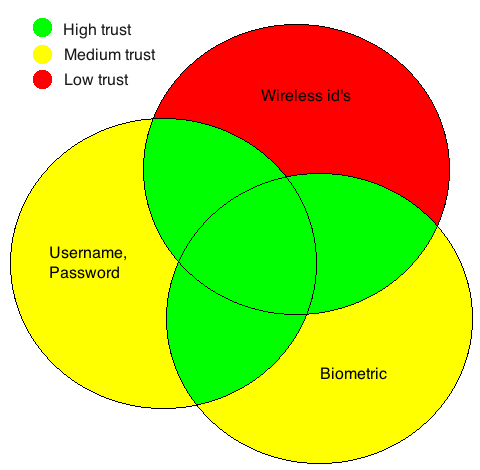
\includegraphics[width=2.5in]{img/authenticationModel}
%	\caption{ Partial login and trust }
%	\label{fig_authentication_model}
%\end{figure}
%
%High trust is obtained by authenticating with a combination of two of the three authentication methods.
%As shown in \cref{table_data_access} a user is only able to view and edit sensitive data within the high trust area of the model.
%
%Medium trust is obtained by authenticating with either a username/password or biometric authentication.
%These two authentication methods is reasonable secure and are used universally for authentication.
%A user that has obtained medium trust is able to view sensitive data but cannot edit or delete it.
%With medium trust a user can view and edit non sensitive data.
%
%Low trust is obtained by calm authentication with a Bluetooth enabled device.
%A user with low trust can view personal non sensitive data like a name or a personal todo-list.
%No edit or delete is allowed.
%
%This model allows the user to be partially authenticated before any physical interaction.
%The system gets the ability to recognize users and may for instance use that information to move a session started on one system to the current system so the user is able to seamlessly work on from the point the previous session ended.
%
%\begin{table}[!t]
%\caption{Data access}
%\label{table_data_access}
%\centering
%% Some packages, such as MDW tools, offer better commands for making tables
%% than the plain LaTeX2e tabular which is used here.
%\begin{tabular}{|p{1.3cm}|p{2.0cm}|p{2.0cm}|p{2.0cm}|}
%\hline
%\textbf{Trust} & \textbf{Non sensitive personal data} & \textbf{Non sensitive data} & \textbf{Sensitive data}\\
%\hline
%\textbf{High} & Read/Write & Read/Write & Read/Write\\
%\hline
%\textbf{Medium} & Read/Write & Read/Write & Read\\
%\hline
%\textbf{Low} & Read & - & -\\
%\hline
%\end{tabular}
%\end{table}
%

	\section{Methods}

\subsection{Existing methods}

\subsubsection{Time of Arrival (ToA)} %This sections needs more work, depending on how much descusion we need futhor on
This technology should be considered, it provides a method for measuring distance more accurately.
The technique uses the travel speed of the wireless signal to measure how far the signal travelled.
This can provide a much more accurate distance, but also has higher requirements for hardware.
It requires time synchronization which works best if hardware supported.

Support on phones and similar devices are very limited, which is why we have chosen not to look further into this method. %need ref to support claim

\url{http://en.wikipedia.org/wiki/Time_of_arrival}

\subsection{Proposed methods}

\subsection{RSSI proximity detection}

\begin{figure}[!t]
	\centering
	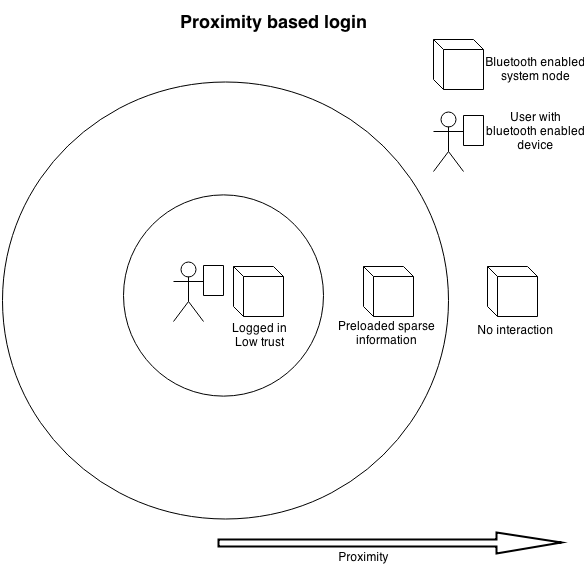
\includegraphics[width=2.5in]{img/proximityBasedLogin}
	\caption{ Proximity based login }
	\label{fig_proximity_based_login}
\end{figure}

It is hard to convert RSSI values into distance because of it's fluctuating nature and the effect of the surrounding environment. Thus instead of dealing in distances the way proximity is detected in this system is by a predefined RSSI value treshold. By determining this threshold and using filters to remove noise it is possible to use RSSI as a means for proximity detection.

When the strength of a RSSI signal reaches the predefined high threshold, when measured from the system, the user is sufficiently close to interact with the system, and the user will be partially authenticated.
When a user has been authenticated but decides to move away from the system the user will be deauthenticated when the RSSI reaches a predefined low threshold.

Furthermore it is possible to preload information about earlier sessions when a user is moving towards the system.
When the user is close enough to be partially authenticated the system thus has preloaded information and may be able to present additional relevant data based on the preloaded information from earlier sessions. 
\cref{fig_proximity_based_login} illustrates the concept of preloading information based on the users proximity to the system.

\subsection{Noise reduction filters}
In order to reduce the noise of the RSSI measurements a standard mean-filter was added to the system.

\subsection{Bluetooth Low Energy authentication}

\subsection{Partial authentication model}
A login method has been developed to take different levels of trust into account.
As presented in \cref{fig_authentication_model} the authentication model has three levels of trust
\begin{itemize}
\item High (green)
\item Medium (yellow)
\item Low (red)
\end{itemize}

\begin{figure}[!t]
	\centering
	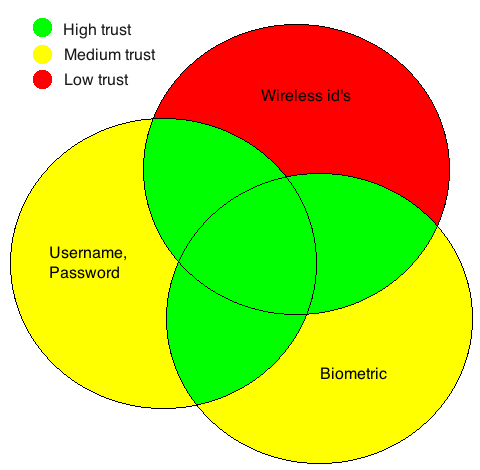
\includegraphics[width=2.5in]{img/authenticationModel}
	\caption{ Partial login and trust }
	\label{fig_authentication_model}
\end{figure}

High trust is obtained by authenticating with a combination of two of the three authentication methods.
As shown in \cref{table_data_access} a user is only able to view and edit sensitive data within the high trust area of the model.

Medium trust is obtained by authenticating with either a username/password or biometric authentication.
These two authentication methods is reasonable secure and are used universally for authentication.
A user that has obtained medium trust is able to view sensitive data but cannot edit or delete it.
With medium trust a user can view and edit non sensitive data.

Low trust is obtained by calm authentication with a Bluetooth enabled device.
A user with low trust can view personal non sensitive data like a name or a personal todo-list.
No edit or delete is allowed.

This model allows the user to be partially authenticated before any physical interaction.
The system gets the ability to recognize users and may for instance use that information to move a session started on one system to the current system so the user is able to seamlessly work on from the point the previous session ended.

\begin{table}[!t]
\caption{Data access}
\label{table_data_access}
\centering
% Some packages, such as MDW tools, offer better commands for making tables
% than the plain LaTeX2e tabular which is used here.
\begin{tabular}{|p{1.3cm}|p{2.0cm}|p{2.0cm}|p{2.0cm}|}
\hline
\textbf{Trust} & \textbf{Non sensitive personal data} & \textbf{Non sensitive data} & \textbf{Sensitive data}\\
\hline
\textbf{High} & Read/Write & Read/Write & Read/Write\\
\hline
\textbf{Medium} & Read/Write & Read/Write & Read\\
\hline
\textbf{Low} & Read & - & -\\
\hline
\end{tabular}
\end{table}
\section{Experiments}

\subsection{Test setup}

Our method requires the phone to be able to use the BLE peripheral role, and the server needs to be able to use the central role.

The specific devices used are an iPhone 5 or a Nexus 5, as mobile device and a Raspberry Pi with a Logilink USB Bluetooth 4.0 dongle running Raspbian Linux\cite{ref:raspbian} as base station. See \cref{fig_solution_overview} for an overview.

The base station test system is build as a prototype using node.js\cite{ref:node} and the Noble node module.
On the iPhone 5 we used the app LightBlue\cite{ref:Lightblue} to advertise a BLE peripheral service.

Currently BLE is amongst other supported by a number of cell phones and wearables. 
The devices tested during this research project is presented in \cref{table:devices}.

\begin{table}[!t]
\caption{Device descriptions}
\label{table:devices}
\centering
% Some packages, such as MDW tools, offer better commands for making tables
% than the plain LaTeX2e tabular which is used here.
\begin{tabular}{|p{2.3cm}|p{1.3cm}|p{3.9cm}|}
\hline
\textbf{Device} & \textbf{Hardware Support} & \textbf{Software Support}\\
\hline
iPhone 5, iPhone 5s (IOS7) & Yes & Yes\\
\hline
Nexus 5 \newline (Kitkat 4.4.2) & Yes & Partial \newline
Central role (Android 4.3)  \newline
peripheral role (Android~L)\\
\hline
Pebble Smartwatch (Pebble OS 2.0) & Yes & Peripheral role\\
\hline
Raspberry Pi (Raspian Linux) and Logilink USB Bluetooth 4.0 dongle & Yes & Yes using BlueZ stack version $\geq$ 5.0 and kernel $\geq$ 3.4\\
\hline

\end{tabular}
\end{table}

%For more information see appendix \ref{appendix:codeused}

\subsection{Scenarios}

%The base scenario consists of a Raspberry Pi with custom software as the system.
The following experiment was conducted with the base station being static throughout the experiments.

A "noisy environment" is an environment with several wifi hotspots and many people moving around with phones having access to Bluetooth, data, etc.

A "regular environment" is a standard home environment.

During the experiments there was always a clear line of sight from the mobile phone to the base station. There was no interference by physical objects or humans between the mobile phone and the base station.

%The device in the test scenario is an iPhone 5 cell phone and other wearables and will be both static and moving depending on the test scenario.

\subsubsection{Dynamic distance}
\label{section:MovingTowardsSystem}
In order for nearby authentication to work a threshold, that determines if the user is close enough for authentication, must be set.

The purpose of this scenario is to observe the relation between distance and RSSI value to make it possible to  define  this threshold. This is done by measuring the RSSI value of a single device at different distances, allowing us to define how close the user needs to be in order to be authenticated.

The base station location is constant. The phone is moved towards the system and RSSI values are measured until the device and the base station have the same location. The phone used is an iPhone 5.

This experiment was conducted in an indoor environment.


\subsubsection{Static distance}
\label{section:MovingTowardsSystem}
As mentioned, RSSI values depends on multiple factors like reflections from environment, distance, transmission strength, etc. 

The purpose of this scenario is to measure how much the RSSI value varies from a static distance. We collect data with the phone being approximately 3 meters away from the base station under the entire scenario.

The phone used is a Nexus 5 using Android L and the experiment was conducted in a regular indoor environment and in a noisy indoor environment. The purpose of the change in environment is to see how noise impacts the result.



% !TeX spellcheck = en_GB
\section{Results}
\label{sec_results}

In the following we present the results from the two scenarios.

\subsection{Dynamic distance}

\begin{figure}		
	
	\begin{tikzpicture}
\begin{axis}
[
width=0.8\textwidth,
xlabel=meter,
ylabel=dBm,
xtick={1, 2, 3, 4, 5, 6, 7, 8, 9, 10, 11, 12, 13, 14},
xticklabels={0.5, 1, 2, 3, 4, 6, 8, 10, 12, 14, 16, 18, 20},
boxplot/draw direction=y
]


%"00.5"                                
\buildBoxPlot{-50}{-46}{-59}{-73}{-43} 
%%"00"                                  
%\buildBoxPlot{-26}{-26}{-27}{-30}{-25} 
%"01"                                  
\buildBoxPlot{-55}{-54}{-58}{-63}{-47} 
%"02"                                  
\buildBoxPlot{-55}{-48}{-58}{-79}{-44} 
%"03"                                  
\buildBoxPlot{-63}{-60}{-66}{-85}{-53} 
%"04"                                  
\buildBoxPlot{-63}{-60}{-68}{-89}{-51} 
%%"05"                                  
%\buildBoxPlot{-68}{-65}{-71}{-84}{-59} 
%"06"                                  
\buildBoxPlot{-69}{-67}{-71}{-90}{-61} 
%%"07"                                  
%\buildBoxPlot{-73}{-68}{-78}{-92}{-63} 
%"08"                                  
%\buildBoxPlot{-73}{-68}{-77}{-90}{-60} 
%%"09"                                  
\buildBoxPlot{-69}{-64}{-71}{-91}{-59} 
%"10"                                  
\buildBoxPlot{-71}{-67}{-75}{-92}{-62} 
%"12"                                  
\buildBoxPlot{-78}{-75}{-82}{-94}{-66} 
%"14"                                  
\buildBoxPlot{-70}{-68}{-73}{-81}{-60} 
%"16"                                  
\buildBoxPlot{-69}{-68}{-77}{-93}{-63} 
%"18"                                  
\buildBoxPlot{-75}{-71}{-78}{-93}{-65} 
%"20"                                  
\buildBoxPlot{-77}{-74}{-80}{-91}{-66} 


\addplot[thick, red] coordinates {
	(1  ,-50)
	(2  ,-55)
	(3  ,-55)
	(4  ,-63)	
	(5  ,-63)	
	(6  ,-69)	
	(7  ,-69)
	(8  ,-71)
	(9  ,-78)
	(10 ,-70)
	(11 ,-69)
	(12 ,-75)
	(13 ,-77)
	
	};
\end{axis}


\end{tikzpicture}
	
	\caption{ Dynamic distance measurements 1 }
	\label{graf_hopper1}
	
\end{figure}

\begin{figure}		
	
	\begin{tikzpicture}
\begin{axis}
[
xlabel=meter,
ylabel=dBm,
xtick={1, 2, 3, 4, 5, 6, 7, 8, 9, 10, 11, 12, 13, 14},
xticklabels={0.5, 1, 2, 3, 4, 6, 8, 10, 12, 14, 16, 18, 20},
boxplot/draw direction=y
]


%%"00"
%\buildBoxPlot{-19}{-18}{-22}{-23}{-18}
%"00.5"
\buildBoxPlot{-43}{-42}{-45}{-49}{-41}
%"01"
\buildBoxPlot{-50}{-48}{-52}{-63}{-44}
%"02"
\buildBoxPlot{-58}{-53}{-62}{-81}{-46}
%"03"
\buildBoxPlot{-61}{-58}{-65}{-86}{-49}
%%"05"
%\buildBoxPlot{-64}{-62}{-66}{-80}{-55}
%"04"
\buildBoxPlot{-63}{-58}{-66}{-85}{-52}
%"06"
%\buildBoxPlot{-62}{-59}{-70}{-78}{-53}
%%"07"
\buildBoxPlot{-65}{-61}{-67}{-83}{-51}
%"08"
%\buildBoxPlot{-70}{-68}{-74}{-89}{-60}
%%"09"
\buildBoxPlot{-73}{-70}{-77}{-92}{-62}
%"12"
\buildBoxPlot{-62}{-61}{-64}{-75}{-57}
%"10"
\buildBoxPlot{-65}{-62}{-70}{-90}{-57}
%"16"
\buildBoxPlot{-63}{-62}{-65}{-71}{-56}
%"20"
\buildBoxPlot{-71}{-71}{-72}{-85}{-67}
%"14"
\buildBoxPlot{-68}{-64}{-71}{-81}{-57}
%"18"
\buildBoxPlot{-75}{-73}{-80}{-91}{-69}


\addplot[thick, red] coordinates {
	(1  ,-43)
	(2  ,-50)
	(3  ,-58)	
	(4  ,-61)	
	(5  ,-63)	
	(6  ,-65)
	(7  ,-73)
	(8  ,-62)
	(9 ,-65)
	(10 ,-63)
	(11 ,-71)
	(12 ,-68)
	(13 ,-75)
		
};

\end{axis}

\end{tikzpicture}
	
	\caption{ Dynamic distance measurements 2 }
	\label{graf_hopper2}
	
\end{figure}

\begin{figure}		
	
	\begin{tikzpicture}
\begin{axis}
[
xlabel=meter,
ylabel=dBm,
xtick={1, 2, 3, 4, 5, 6, 7, 8, 9, 10, 11, 12, 13, 14},
xticklabels={0.5, 1, 2, 3, 4, 6, 8, 10, 12, 14, 16, 18, 20},
boxplot/draw direction=y
]


%%"00"                                   
%\buildBoxPlot{-36}{-31}{-39}{-43}{-30}  
%"00.5"                                 
\buildBoxPlot{-55}{-50}{-61}{-83}{-46}  
%"01"                                   
\buildBoxPlot{-49}{-47}{-62}{-81}{-41}  
%"02"                                   
\buildBoxPlot{-55}{-51}{-59}{-77}{-46}  
%"03"                                   
\buildBoxPlot{-66}{-60}{-71}{-76}{-57}  
%"04"                                   
\buildBoxPlot{-60}{-55}{-62}{-65}{-52}  
%%"05"                                   
%\buildBoxPlot{-65}{-63}{-68}{-88}{-58}  
%"06"                                   
\buildBoxPlot{-66}{-65}{-68}{-78}{-59}  
%%"07"                                   
%\buildBoxPlot{-69}{-66}{-74}{-83}{-62}  
%"08"                                   
\buildBoxPlot{-63}{-62}{-75}{-83}{-59}  
%%"09"                                   
%\buildBoxPlot{-65}{-61}{-67}{-69}{-57}  
%"10"                                   
\buildBoxPlot{-63}{-62}{-65}{-72}{-57}  
%"12"                                   
\buildBoxPlot{-66}{-64}{-68}{-78}{-59}  
%"14"                                   
\buildBoxPlot{-67}{-66}{-69}{-91}{-63}  
%"16"                                   
\buildBoxPlot{-69}{-67}{-71}{-87}{-59}  
%"18"                                   
\buildBoxPlot{-73}{-71}{-76}{-88}{-65}  
%"20"                                   
\buildBoxPlot{-75}{-72}{-77}{-91}{-67}  


\addplot[thick, red] coordinates {
	(1  ,-55)
	(2  ,-49)
	(3  ,-55)	
	(4  ,-66)	
	(5  ,-60)	
	(6  ,-66)
	(7  ,-63)
	(8  ,-63)
	(9 ,-66)
	(10 ,-67)
	(11 ,-69)
	(12 ,-73)
	(13 ,-75)
	
};

\end{axis}

\end{tikzpicture}
	
	\caption{ Dynamic distance measurements 3 }
	\label{graf_hopper3}
	
\end{figure}

\begin{figure}		
	
	\begin{tikzpicture}
\begin{axis}
[
xlabel=meter,
ylabel=dBm,
xtick={1, 2, 3, 4, 5, 6, 7, 8, 9, 10, 11, 12, 13, 14},
xticklabels={0.5, 1, 2, 3, 4, 6, 8, 10, 12, 14, 16, 18, 20},
boxplot/draw direction=y
]


%%"00"                                 
%\buildBoxPlot{-13}{-12}{-15}{-16}{-10}
%"00.5"                               
\buildBoxPlot{-46}{-44}{-47}{-51}{-41}
%"01"                                 
\buildBoxPlot{-62}{-60}{-70}{-91}{-52}
%"02"                                 
\buildBoxPlot{-61}{-60}{-62}{-71}{-53}
%"03"                                 
\buildBoxPlot{-67}{-61}{-71}{-77}{-55}
%"04"                                 
\buildBoxPlot{-65}{-64}{-67}{-84}{-60}
%%"05"                                 
%\buildBoxPlot{-72}{-69}{-75}{-93}{-65}
%"06"                                 
\buildBoxPlot{-68}{-64}{-71}{-76}{-62}
%%"07"                                 
%\buildBoxPlot{-71}{-69}{-75}{-80}{-65}
%"08"                                 
\buildBoxPlot{-71}{-68}{-74}{-84}{-65}
%%"09"                                 
%\buildBoxPlot{-71}{-68}{-79}{-91}{-65}
%"10"                                 
\buildBoxPlot{-71}{-71}{-72}{-77}{-67}
%"12"                                 
\buildBoxPlot{-70}{-67}{-73}{-75}{-64}
%"14"                                 
\buildBoxPlot{-77}{-75}{-80}{-94}{-63}
%"16"                                 
\buildBoxPlot{-71}{-70}{-75}{-84}{-68}
%"18"                                 
\buildBoxPlot{-78}{-75}{-86}{-92}{-69}
%"20"                                 
\buildBoxPlot{-82}{-79}{-83}{-93}{-72} 


\addplot[thick, red] coordinates {
	(1  ,-46)
	(2  ,-62)
	(3  ,-61)	
	(4  ,-67)	
	(5  ,-65)	
	(6  ,-68)
	(7  ,-71)
	(8  ,-71)
	(9 ,-70)
	(10 ,-77)
	(11 ,-71)
	(12 ,-78)
	(13 ,-82)
	
};

\end{axis}

\end{tikzpicture}
	
	\caption{ Dynamic distance measurements 4 }
	\label{graf_hopper4}
	
\end{figure}

%\begin{figure}		
%	
%	\begin{tikzpicture}
  \begin{axis}
    [
	xlabel=meter,
	ylabel=dBm,
	xtick={1, 2, 3, 4, 5, 6, 7, 8, 9, 10, 11, 12},
    xticklabels={0, 2, 4, 6, 8, 10, 12, 14, 16, 18, 20},
    boxplot/draw direction=y
    ]
    

%"00,0"
\buildBoxPlot{-46}{ -45}{ -59}{ -63}{ -44}
%"00,5"
%\buildBoxPlot{-55}{ -55}{ -58}{ -60}{ -54}
%"01"
%\buildBoxPlot{-68}{ -67}{ -69}{ -72}{ -65}
%"02"
\buildBoxPlot{-70}{ -68}{ -74}{ -78}{ -65}
%"04"
\buildBoxPlot{-69}{ -69}{ -71}{ -72}{ -67}
%"06"
\buildBoxPlot{-78}{ -77}{ -78}{ -79}{ -73}
%"08"
\buildBoxPlot{-78}{ -77}{ -83}{ -83}{ -76}
%"10"
\buildBoxPlot{-78}{ -77}{ -79}{ -81}{ -75}
%"12"
\buildBoxPlot{-80}{ -78}{ -81}{ -84}{ -76}
%"14"
\buildBoxPlot{-77}{ -76}{ -77}{ -78}{ -75}
%"18"
\buildBoxPlot{-85}{ -83}{ -85}{ -89}{ -81}
%"16"
\buildBoxPlot{-81}{ -80}{ -81}{ -83}{ -78}
%"20"
\buildBoxPlot{-84}{ -83}{ -84}{ -87}{ -82}


\end{axis}
	
\end{tikzpicture}

%	
%	\caption{ Dynamic distance measurements Filtered }
%	\label{graf_DynamicMesurementsFiltered}
%	
%\end{figure}

The data from this scenario is presented in \cref{graf_hopper1} to \cref{graf_hopper4}.
The figure shows RSSI value at 2 meter intervals between the base station and the mobile phone.
If we look at the median of the measurements there seems to be an exponential decreasing relation between distance and RSSI value.
We also see that measurements on the low side of the mean values has a wider distribution than on the high side of the mean measurements.

\subsection{Static distance}
\begin{figure}
	\begin{tikzpicture}
\begin{axis}[
width=0.8\textwidth,
ymax=0.5,
xlabel=dBm,
ylabel=probability density]
\addplot[blue!20!blue] coordinates {
	(-91 ,0.0001093255)
	(-90 ,0.0013119055)
	(-89 ,0.0017492074)
	(-88 ,0.0024051602)
	(-87 ,0.0068875041)
	(-86 ,0.0072154805)
	(-85 ,0.0084180606)
	(-84 ,0.0134470318)
	(-83 ,0.0109325462)
	(-82 ,0.0147589374)
	(-81 ,0.0274406909)
	(-80 ,0.028643271)
	(-79 ,0.0256914835)
	(-78 ,0.04023177)
	(-77 ,0.0571772166)
	(-76 ,0.0594730513)
	(-75 ,0.1130425276)
	(-74 ,0.1168689188)
	(-73 ,0.0850552094)
	(-72 ,0.0906308079)
	(-71 ,0.0727014322)
	(-70 ,0.0412156991)
	(-69 ,0.0327976386)
	(-68 ,0.0378266098)
	(-67 ,0.0256914835)
	(-66 ,0.0301738275)
	(-65 ,0.0387012135)
	(-64 ,0.0072154805)
	(-63 ,0.0015305565)
	(-62 ,0.0006559528)

		};
\addplot[red!20!red] coordinates {
	(-91, 0)
	(-87, 0.0001107297)
	(-86, 0.0001107297)
	(-83, 0.0001107297)
	(-82, 0.0003321891)
	(-81, 0.0006643783)
	(-80, 0.0011072971)
	(-79, 0.0006643783)
	(-78, 0.0014394862)
	(-77, 0.0014394862)
	(-76, 0.0019931348)
	(-75, 0.0115158897)
	(-74, 0.0627837449)
	(-73, 0.0628944746)
	(-72, 0.1308825158)
	(-71, 0.1755065884)
	(-70, 0.3232200199)
	(-69, 0.1824825601)
	(-68, 0.0367622633)
	(-67, 0.0046506478)
	(-66, 0.0005536485)
	(-64, 0.000775108)
	(-54, 0)
	};
\legend{Noisy Env,Quiet Env}
\end{axis}
\end{tikzpicture}

	
	\caption{Static distance measurements}
	\label{graf_StaticMesurements}
\end{figure}

The data from this scenario is presented in \cref{graf_StaticMesurements}.
The figure shows how measurements are distributed over a period of 20 minutes when the distance between the base station and the mobile phone is static.
The experiment was performed in a quiet and a noisy environment.
As one would expect the RSSI values has a much higher spread in the noisy environment than in the quiet environment. 
 

\section{Discussion}
Seeing how the value of the RSSI measured from the device fluctuates in \cref{graf_hopper1} to \cref{graf_hopper4} it is clear that RSSI is hard to use for distance measurements.
From a mean around 45 when measured right on top of the system the RSSI value drops drastically within the first few meters.
As the device moves further away from the system the RSSI value becomes lower but there is no apparent model to the decline.

The noise seams to fluctuate more towards the noise side of the mean. This suggests that if a lower value is measured it is more reliable then a high value, witch fits in well for authentication purposes.
Since most outliers are in the lower dBm end, there is a greater chance that you will be incorrectly logged out as a result of noise than incorrectly logged in.

Looking at \cref{graf_StaticMesurements} we clearly see that the RSSI value becomes less reliable the more noise there is in the environment.
The Noise level will affect how the hysteresis thresholds should be configured.
With too much noise in the environment the mean value of the graph will become indistinct from the rest.




\section{Conclusion}
Using RSSI value as viable means for proximity detection is possible but inaccurate. Therefore we implemented a solution which uses a filter and a hysteresis threshold combined, to remove noise from RSSI measurements and optimize accuracy and thereby make a more consistent proximity detection.

RSSI values depends on multiple factors, such as distance, reflections from environment, transmission strength, etc., which is reflected in our test results.
Environment knowledge prior to implementing authentication using RSSI values is therefore crucial to be able to calibrate the base station correctly. 
Even when the base station is calibrated there is the possibility of interference of for instance people moving between the mobile phone and the base station. 
This adds a layer of inaccuracy to the system which is really hard to predict and therefore take into account when doing proximity detection.

We have developed an application that is capable of proximity detecting of a BLE device running with the peripheral role. This is done using the RSSI value witch is being broadcasted by the device.

Because RSSI measurements are significantly effected by the environment, hysteresis thresholds must be used and calibrated with respect to the environment.
We have found that this method makes authentication possible using BLE, however for a highly secured system this method might not be secure enough.

Source code is available on Github:
\url{https://github.com/KrauseStefan/ReserchProject-RSSI-Login/tree/master/testApp}.

%
%A partial authentication model has been proposed taking the security aspect of calm authentication into consideration. The model has three levels of trust: Low, Medium and High allowing different read/write/edit rights according to the level of trust.

%We have shown that context aware authentication using Bluetooth Low Energy is possible using RSSI measurements for proximity detection.

\section{Future work}
The following experiments would be interesting to consider for future work.


\subsection{Device RSSI value differences}

During this project we did not look into whether switching phone device would have an impact on the measured RSSI values.


\subsection{Multiple devices}

The possibility of two users moving towards the same system is appearent. Therefor, to test how the RSSI value varies when multiple devices are near the system would be interesting.


\subsection{Time of Arrival (ToA)}
ToA is a method for measuring the distance between two objects, by measuring the time it takes a radio signal to travel between the objects. This is the same technique used in gps. ToA can provide reliable distance measurements but requires special hardware. This might serve as an interesting alternative to using the RSSI value of a Bluetooth device.



% if have a single appendix:
%\appendix[Proof of the Zonklar Equations]
% or
%\appendix  % for no appendix heading
% do not use \section anymore after \appendix, only \section*
% is possibly needed

% use appendices with more than one appendix
% then use \section to start each appendix
% you must declare a \section before using any
% \subsection or using \label (\appendices by itself
% starts a section numbered zero.)
%


%\appendices


%% use section* for acknowledgement
%\ifCLASSOPTIONcompsoc
%  % The Computer Society usually uses the plural form
%  \section*{Acknowledgments}
%\else
%  % regular IEEE prefers the singular form
%  \section*{Acknowledgment}
%\fi
%

%The authors would like to thank...


% Can use something like this to put references on a page
% by themselves when using endfloat and the captionsoff option.
%\ifCLASSOPTIONcaptionsoff
%  \newpage
%\fi

\backmatter

% references section

% can use a bibliography generated by BibTeX as a .bbl file
% BibTeX documentation can be easily obtained at:
% http://www.ctan.org/tex-archive/biblio/bibtex/contrib/doc/
% The IEEEtran BibTeX style support page is at:
% http://www.michaelshell.org/tex/ieeetran/bibtex/
%\bibliographystyle{IEEEtran}
% argument is your BibTeX string definitions and bibliography database(s)
%\bibliography{IEEEabrv,../bib/paper}
%
% <OR> manually copy in the resultant .bbl file
% set second argument of \begin to the number of references
% (used to reserve space for the reference number labels box)
\begin{thebibliography}{1}

\bibitem{ref:Takashi}
 Kikawa, Yoshikawa, Ohkubo, Takeshita, Shiraishi and Takahashi:  
 A Presence-detection Method using RSSI of a Bluetooth Device, 2010, International Journal of Informatics Society, VOL. 2, NO. 1. 

%\bibitem{ref:win8_BLE_support}
%Bluetooth Low Energy Overview. Microsoft developer network. Retrieved from http://msdn.microsoft.com/en-us/library/windows/hardware/jj159880(v=vs.85).aspx

\bibitem{ref:Power_usage}
iBeacon Battery Drain on Apple vs Android: A Technical Report. Aislelabs. Retrieved from http://www.aislelabs.com/reports/ibeacon-battery-drain-iphones/

\bibitem{ref:bardram}
E. Bardram. 2005. The trouble with login: on usability and computer security in ubiquitous computing. Personal Ubiquitous Comput. 9, 6 (November 2005), 357-367. DOI=10.1007/s00779-005-0347-6 http://dx.doi.org/10.1007/s00779-005-0347-6

\bibitem{ref:covington}
Covington, Michael J., et al. "A context-aware security architecture for emerging applications." Computer Security Applications Conference, 2002. Proceedings. 18th Annual. IEEE, 2002.

\bibitem{ref:bandara}
Bandara, Udana, et al. "Design and implementation of a bluetooth signal strength based location sensing system." Radio and Wireless Conference, 2004 IEEE. IEEE, 2004.

\bibitem{ref:rssidistance}
Awad, Abdalkarim, Thorsten Frunzke, and Falko Dressler. "Adaptive distance estimation and localization in WSN using RSSI measures." Digital System Design Architectures, Methods and Tools, 2007. DSD 2007. 10th Euromicro Conference on. IEEE, 2007.

\bibitem{ref:node}
Tilkov, Stefan, and Steve Vinoski. "Node. js: Using JavaScript to build high-performance network programs." IEEE Internet Computing 14.6 (2010): 0080-83.

\bibitem{ref:Lightblue}
https://itunes.apple.com/dk/app/lightblue-bluetooth-low-energy/id557428110?mt=8

\bibitem{ref:raspbian}
http://www.raspbian.org/

%H.~Kopka and P.~W. Daly, \emph{A Guide to \LaTeX}, 3rd~ed.\hskip 1em plus
%  0.5em minus 0.4em\relax Harlow, England: Addison-Wesley, 1999.

\end{thebibliography}


% trigger a \newpage just before the given reference
% number - used to balance the columns on the last page
% adjust value as needed - may need to be readjusted if
% the document is modified later
%\IEEEtriggeratref{8}
% The "triggered" command can be changed if desired:
%\IEEEtriggercmd{\enlargethispage{-5in}}

% biography section
% 
% If you have an EPS/PDF photo (graphicx package needed) extra braces are
% needed around the contents of the optional argument to biography to prevent
% the LaTeX parser from getting confused when it sees the complicated
% \includegraphics command within an optional argument. (You could create
% your own custom macro containing the \includegraphics command to make things
% simpler here.)
%\begin{IEEEbiography}[{\includegraphics[width=1in,height=1.25in,clip,keepaspectratio]{mshell}}]{Michael Shell}
% or if you just want to reserve a space for a photo:

\begin{IEEEbiography}[{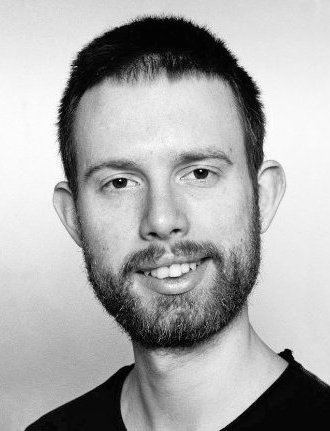
\includegraphics[width=1in,height=1.25in,clip,keepaspectratio]{img/skk.jpg}}]{Stefan Krause-Kj\ae r}
is a 3rd semester Technical IT student at Aarhus University. His primary field of experience is web development and distributed systems.
\end{IEEEbiography}

% if you will not have a photo at all:
\begin{IEEEbiography}[{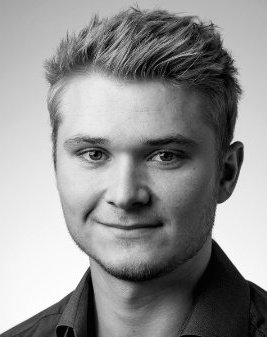
\includegraphics[width=1in,height=1.25in,clip,keepaspectratio]{img/tn.jpg}}]{Theis Nickelsen}
is a 3rd semester M.Sc.Eng. IT student at Aarhus University. Since 2011 he has primarily been engaged in mobile computing and distributed systems.
\end{IEEEbiography}

% insert where needed to balance the two columns on the last page with
% biographies
%\newpage

\begin{IEEEbiography}[{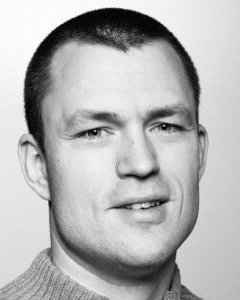
\includegraphics[width=1in,height=1.25in,clip,keepaspectratio]{img/tts.jpg}}]{Thomas Thisgaard Steffensen}
is a 3rd semester M.Sc.Eng. IT student at Aarhus University. His research interests include mobile computing and distributed systems.
\end{IEEEbiography}

% You can push biographies down or up by placing
% a \vfill before or after them. The appropriate
% use of \vfill depends on what kind of text is
% on the last page and whether or not the columns
% are being equalized.

%\vfill

% Can be used to pull up biographies so that the bottom of the last one
% is flush with the other column.
%\enlargethispage{-5in}



% that's all folks
\end{document}

